\documentclass[11pt]{article}
\usepackage[T1]{fontenc}
\usepackage{lmodern}
\usepackage{parskip}
\usepackage[colorlinks=true,urlcolor=Blue,linkcolor=black,citecolor=black]{hyperref}
\usepackage{graphicx}
\usepackage{amsmath}
\usepackage[utf8]{inputenc}
\usepackage[spanish]{babel}
\usepackage{fancyhdr}
\usepackage{csquotes}
\usepackage{lastpage}
\usepackage{array}
\usepackage{listings}
\usepackage{color}
\definecolor{dkgreen}{rgb}{0,0.6,0}
\definecolor{gray}{rgb}{0.5,0.5,0.5}
\definecolor{mauve}{rgb}{0.58,0,0.82}
\usepackage[affil-it]{authblk}
\usepackage[activate={true,nocompatibility},final,tracking=true,kerning=true,spacing=true,factor=1100,stretch=10,shrink=10]{microtype}
\usepackage[hmargin=2cm,top=4cm,headheight=65pt,footskip=65pt]{geometry}
\usepackage{hyperref}
\usepackage{graphicx}
\usepackage{float}
\usepackage{tabularx}
\graphicspath{ {./screenshots/p03/} }

% Documento
\begin{document}

% Título
\title{IFA. Práctica de laboratorio 03}

\author{Hugo Fonseca Díaz \\ email \href{mailto:uo258318@uniovi.es}{uo258318@uniovi.es}}
\affil{Escuela de Ingeniería Informática. Universidad de Oviedo.}

\maketitle

% Ejercicio 1
\section{Ejercicio 1}
Se crea el caso en Autopsy con los datos solicitados.

\begin{figure}[H]
    \caption{Ejercicio 1: Creación del caso}
    \centering
    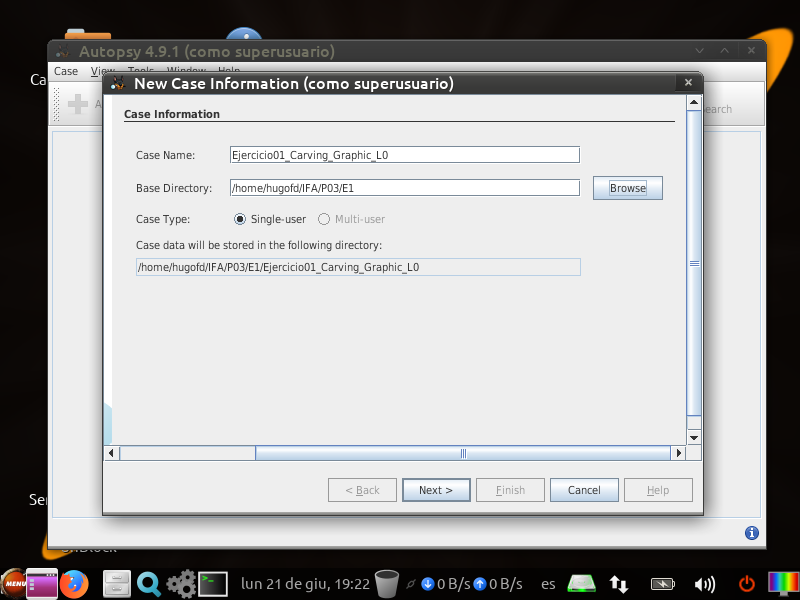
\includegraphics[scale=0.7]{e1-1.png}
\end{figure}

\begin{figure}[H]
    \caption{Ejercicio 1: Detalles del examinador}
    \centering
    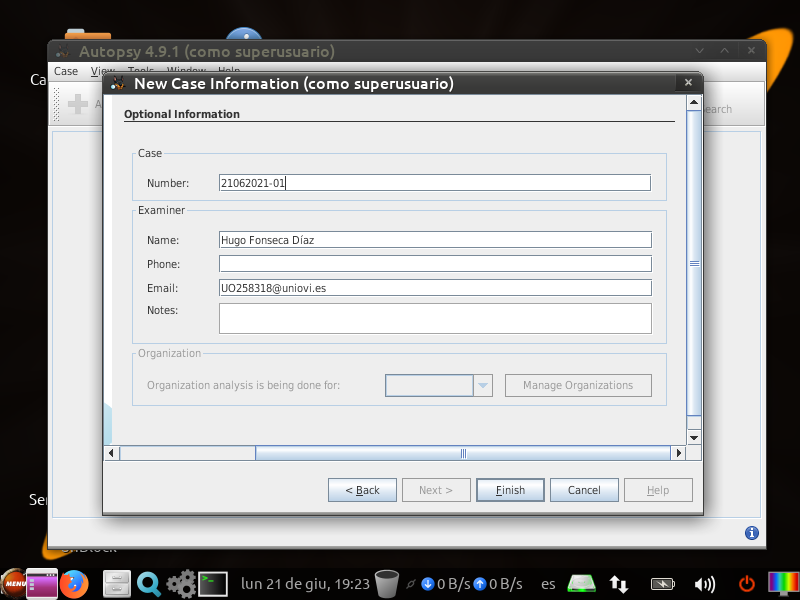
\includegraphics[scale=0.7]{e1-2.png}
\end{figure}

Añadimos la imagen a analizar.

\begin{figure}[H]
    \caption{Ejercicio 1: Selección de la imagen}
    \centering
    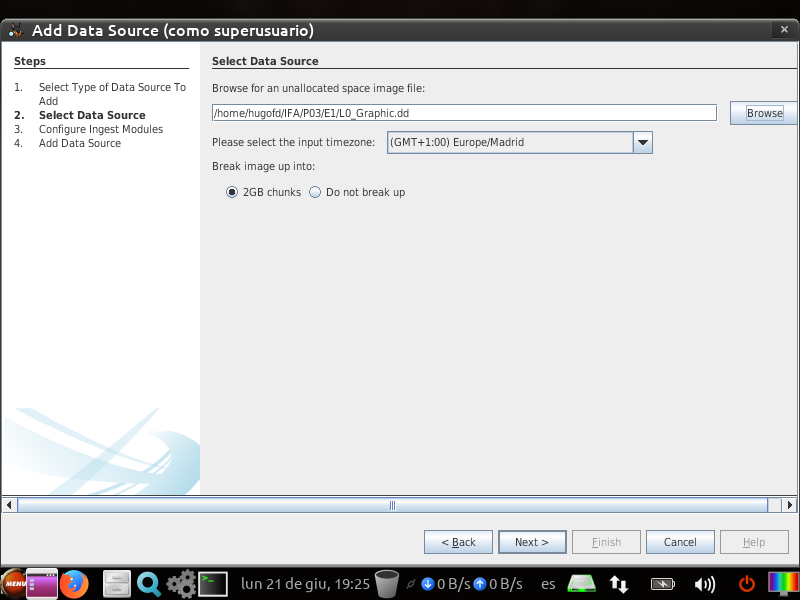
\includegraphics[scale=0.7]{e1-3.png}
\end{figure}

Se seleccionan los módulos de identificación de tipos de fichero, parseador de Exif y \textit{PhotoRec Carver}.

\begin{figure}[H]
    \caption{Ejercicio 1: Selección de módulos}
    \centering
    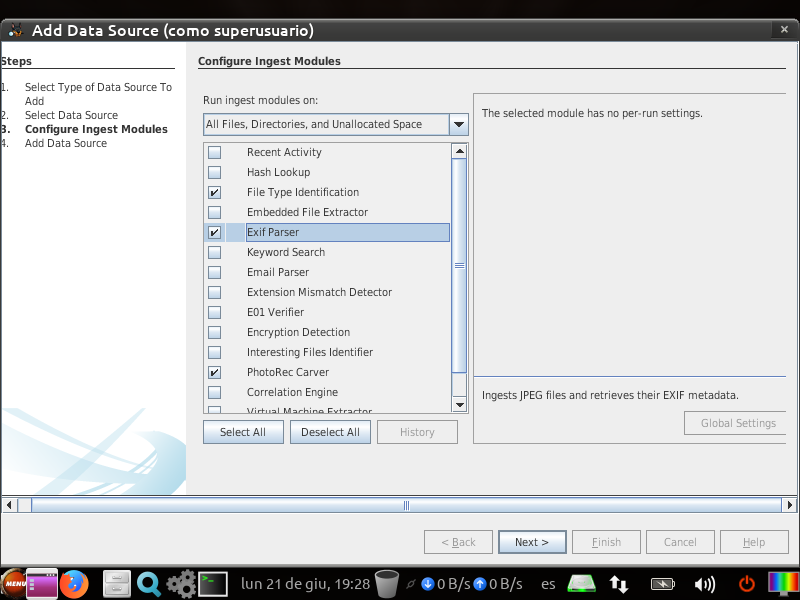
\includegraphics[scale=0.7]{e1-4.png}
\end{figure}

Se ejecuta el análisis y se obtienen los resultados con los que se rellenará la tabla.

\begin{figure}[H]
    \caption{Ejercicio 1: Resultados del análisis}
    \centering
    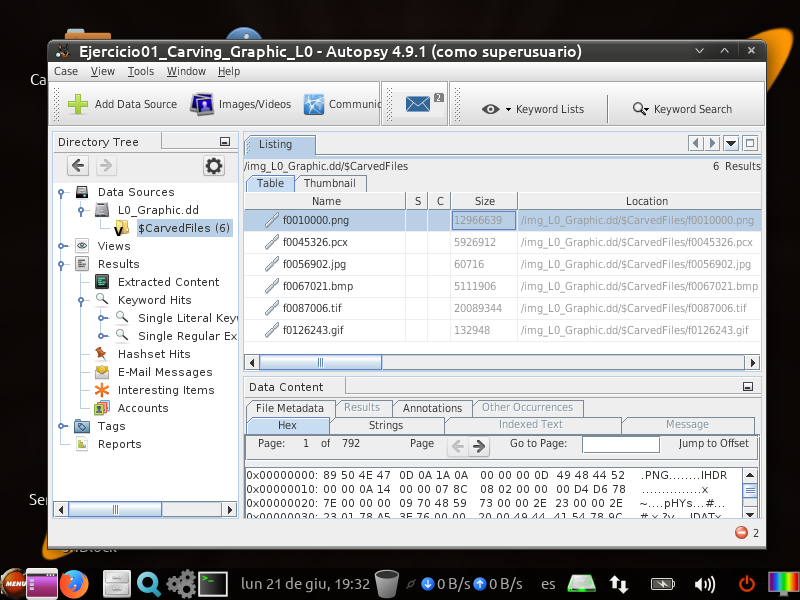
\includegraphics[scale=0.7]{e1-5.png}
\end{figure}

\begin{figure}[H]
    \caption{Ejercicio 1: Imágenes obtenidas}
    \centering
    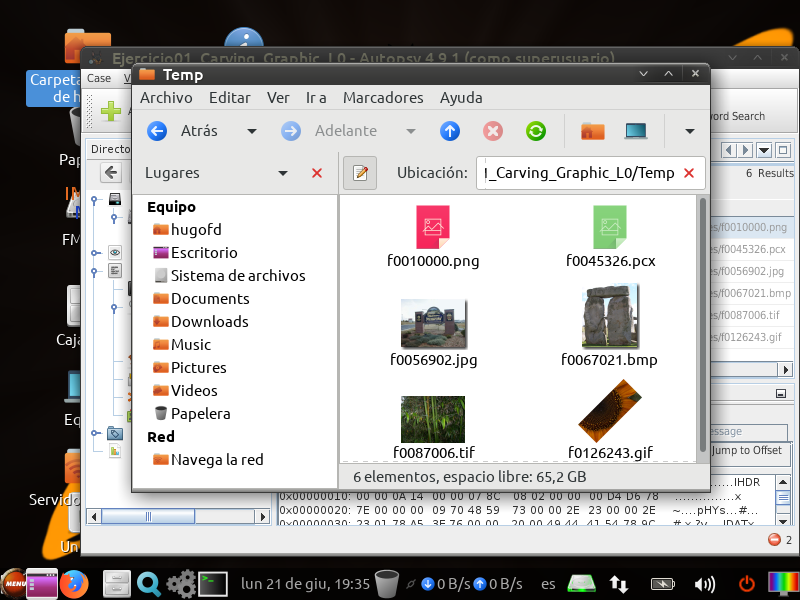
\includegraphics[scale=0.7]{e1-6.png}
\end{figure}

Para abrir el archivo con extensión \textit{pcx} se ha utilizado un visor de imágenes online, al no disponer de uno adecuado en el equipo.

\begin{table}[H]
    \centering
    \begin{tabular}{|c|c|c|}
        \hline
        Nombre del fichero en Autopsy & Tamaño del fichero (en Bytes) & Breve descripción imagen visible \\
        \hline\hline
        f0010000.png & 12966639 & Flor morada \\
        \hline
        f0045326.pcx & 5926912 & Iglesia y fuente \\
        \hline
        f0056902.jpg & 60716 & Cartel 'Welcome to Moscow' \\
        \hline
        f0067021.bmp & 5111906 & Piedras en forma de Pi \\
        \hline
        f0087006.tif & 20089344 & Cañas de bambú \\
        \hline
        f0126243.gif & 132948 & Girasol \\
        \hline
    \end{tabular}
\end{table}

% Ejercicio 2
\section{Ejercicio 2}
Se crea el caso en Autopsy con los datos solicitados.

\begin{figure}[H]
    \caption{Ejercicio 2: Creación del caso}
    \centering
    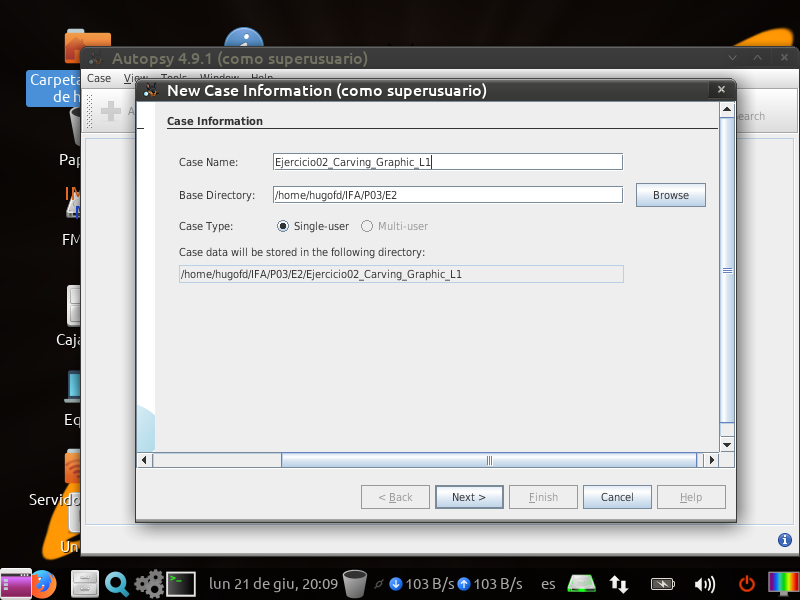
\includegraphics[scale=0.7]{e2-1.png}
\end{figure}

\begin{figure}[H]
    \caption{Ejercicio 2: Detalles del examinador}
    \centering
    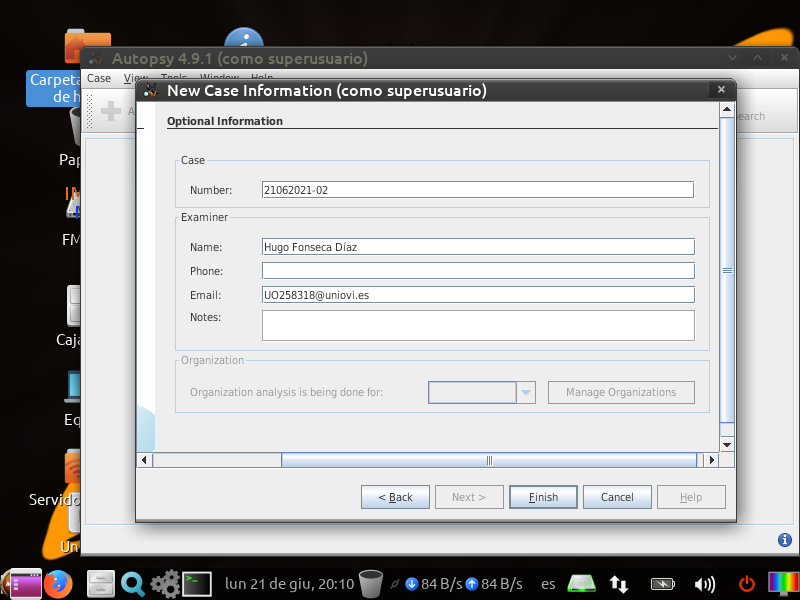
\includegraphics[scale=0.7]{e2-2.png}
\end{figure}

Añadimos la imagen a analizar.

\begin{figure}[H]
    \caption{Ejercicio 2: Selección de la imagen}
    \centering
    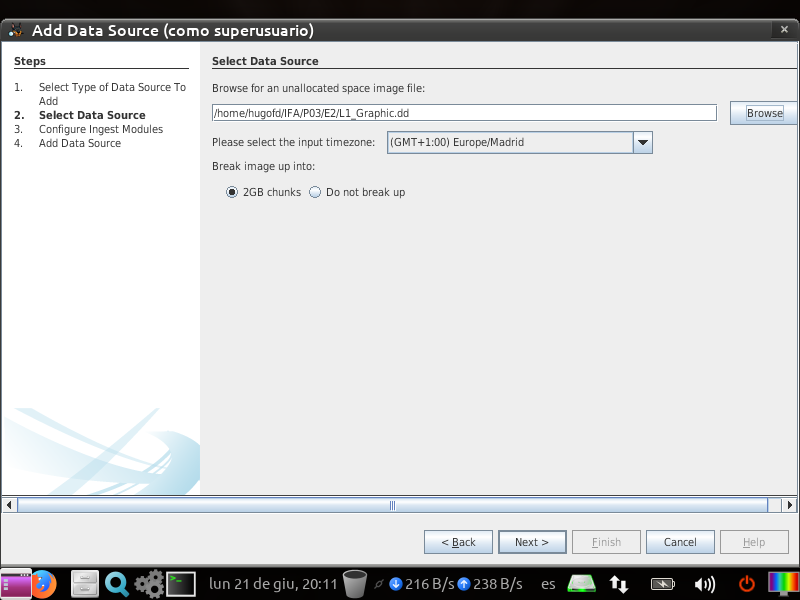
\includegraphics[scale=0.7]{e2-3.png}
\end{figure}

Se seleccionan los módulos de identificación de tipos de fichero, parseador de Exif y \textit{PhotoRec Carver}.

\begin{figure}[H]
    \caption{Ejercicio 2: Selección de módulos}
    \centering
    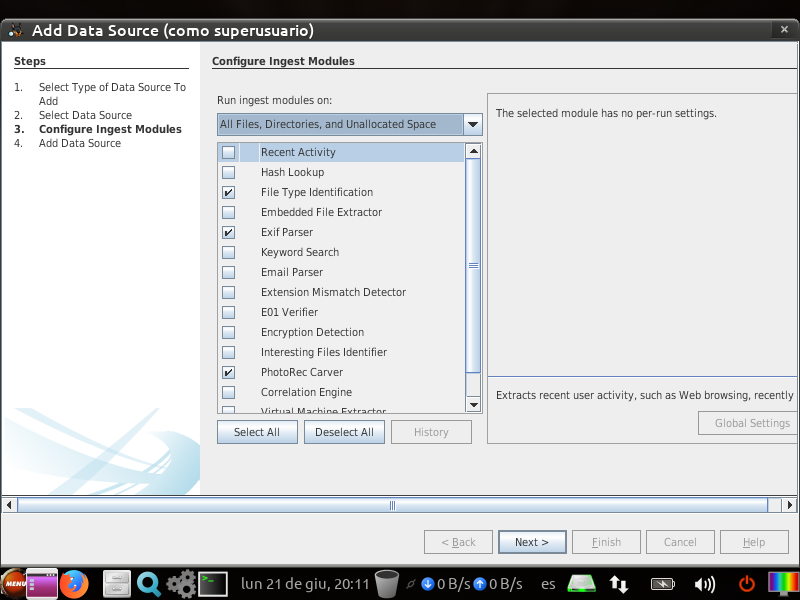
\includegraphics[scale=0.7]{e2-4.png}
\end{figure}

Se ejecuta el análisis y se obtienen los resultados con los que se rellenará la tabla.

\begin{figure}[H]
    \caption{Ejercicio 2: Resultados del análisis}
    \centering
    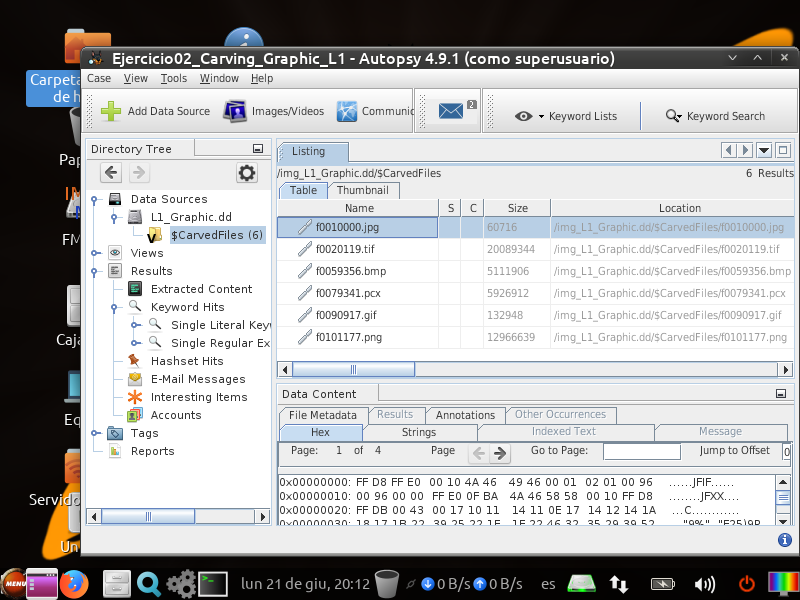
\includegraphics[scale=0.7]{e2-5.png}
\end{figure}

\begin{figure}[H]
    \caption{Ejercicio 2: Imágenes obtenidas}
    \centering
    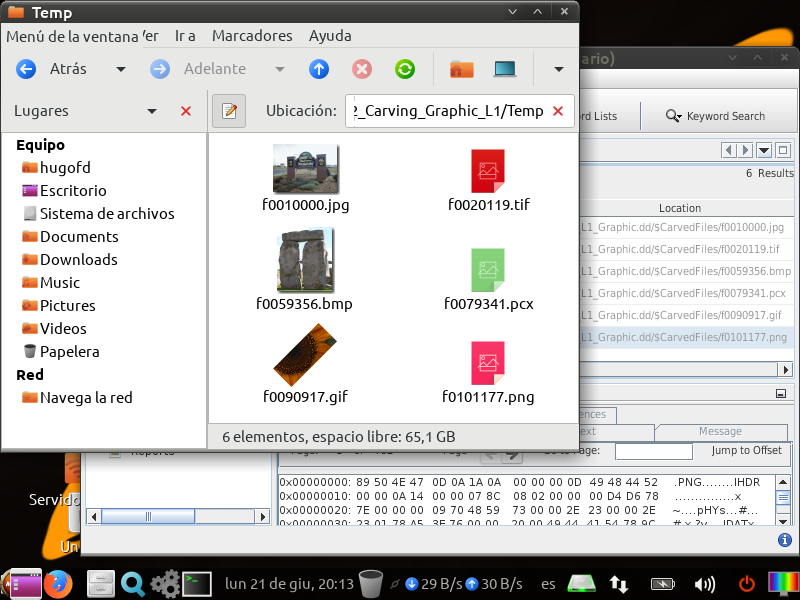
\includegraphics[scale=0.7]{e2-6.png}
\end{figure}

Para abrir el archivo con extensión \textit{pcx} se ha utilizado un visor de imágenes online, al no disponer de uno adecuado en el equipo.

\begin{table}[H]
    \centering
    \begin{tabular}{|c|c|c|}
        \hline
        Nombre del fichero en Autopsy & Tamaño del fichero (en Bytes) & Breve descripción imagen visible \\
        \hline\hline
        f0010000.jpg & 60716 & Cartel 'Welcome to Moscow' \\
        \hline
        f0020119.tif & 20089344 & Cañas de bambú \\
        \hline
        f0059356.bmp & 5111906 & Piedras en forma de Pi \\
        \hline
        f0079341.pcx & 5926912 & Iglesia y fuente \\
        \hline
        f0090917.gif & 132948 & Girasol \\
        \hline
        f0101177.png & 12966639 & Flor morada \\
        \hline
    \end{tabular}
\end{table}

% Ejercicio 3
\section{Ejercicio 3}
Se crea el caso en Autopsy con los datos solicitados.

\begin{figure}[H]
    \caption{Ejercicio 3: Creación del caso}
    \centering
    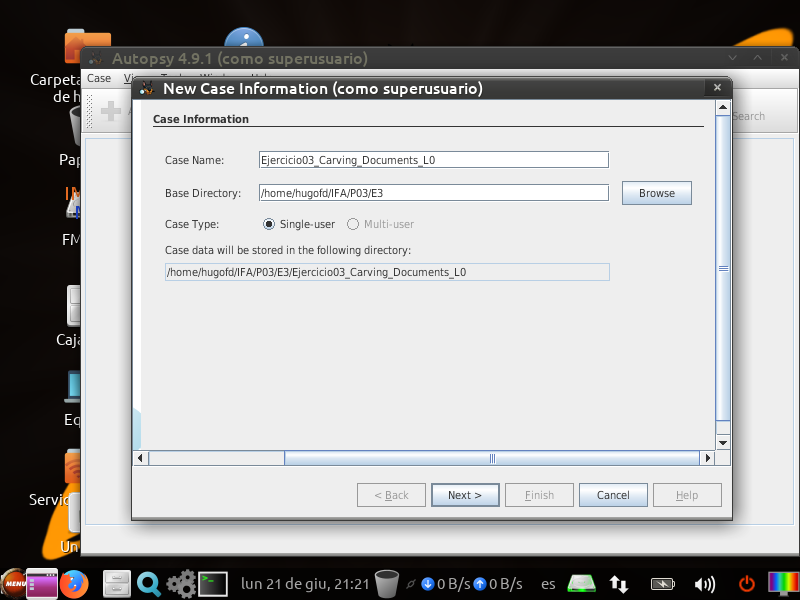
\includegraphics[scale=0.7]{e3-1.png}
\end{figure}

\begin{figure}[H]
    \caption{Ejercicio 3: Detalles del examinador}
    \centering
    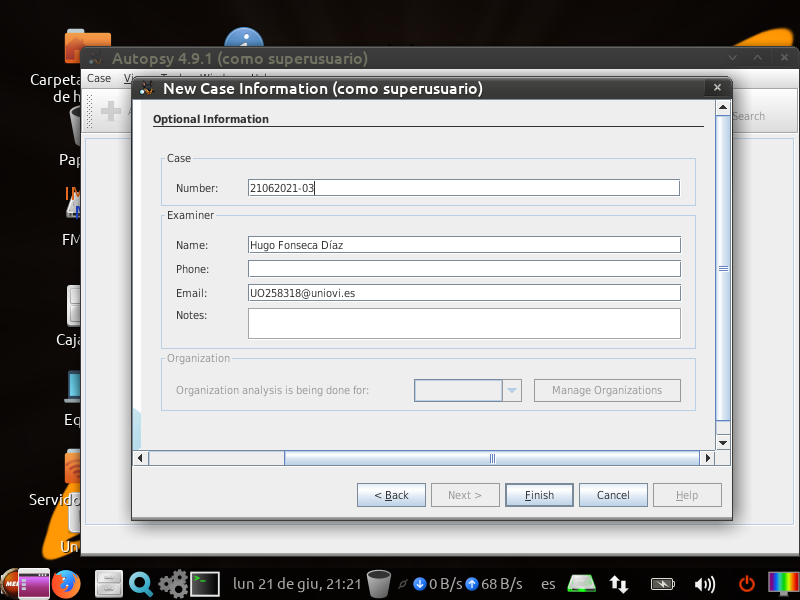
\includegraphics[scale=0.7]{e3-2.png}
\end{figure}

Añadimos la imagen a analizar.

\begin{figure}[H]
    \caption{Ejercicio 3: Selección de la imagen}
    \centering
    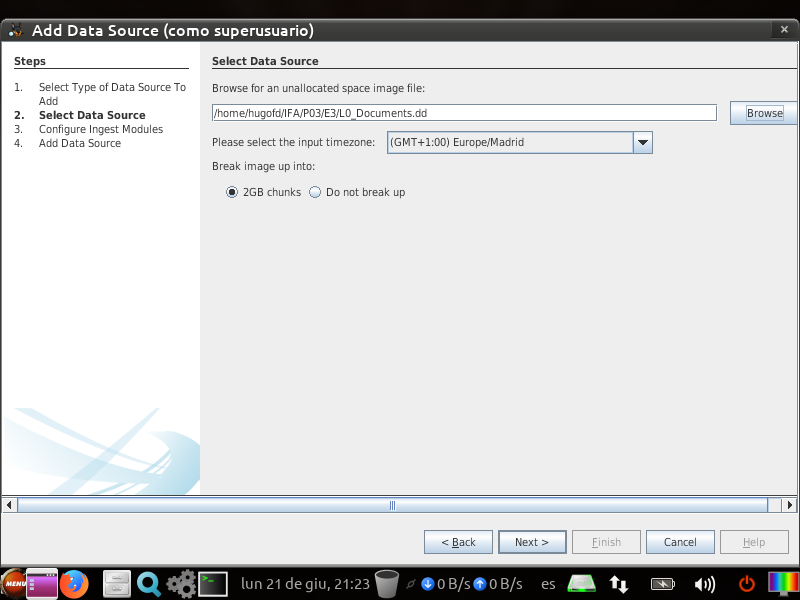
\includegraphics[scale=0.7]{e3-3.png}
\end{figure}

Se seleccionan los módulos de identificación de tipos de fichero, parseador de Exif y \textit{PhotoRec Carver}.

\begin{figure}[H]
    \caption{Ejercicio 3: Selección de módulos}
    \centering
    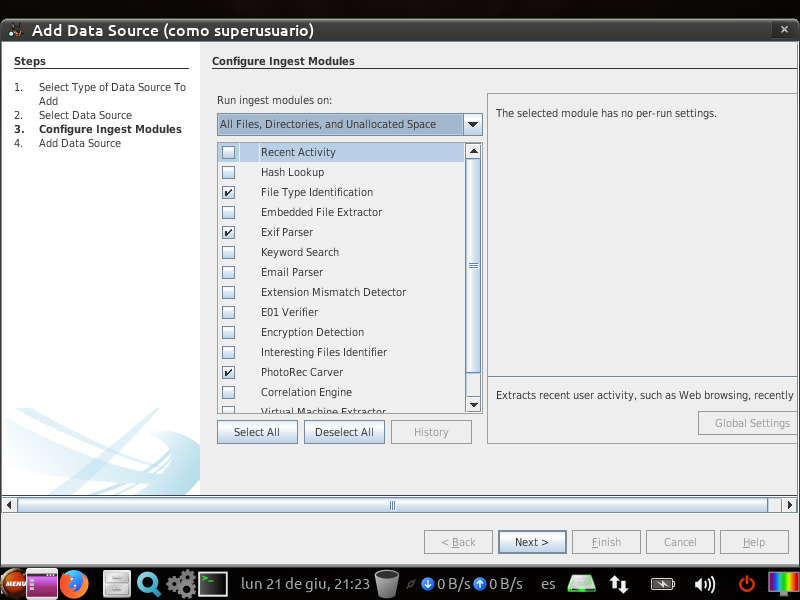
\includegraphics[scale=0.7]{e3-4.png}
\end{figure}

Se ejecuta el análisis y se obtienen los resultados con los que se rellenará la tabla.

\begin{figure}[H]
    \caption{Ejercicio 3: Resultados del análisis}
    \centering
    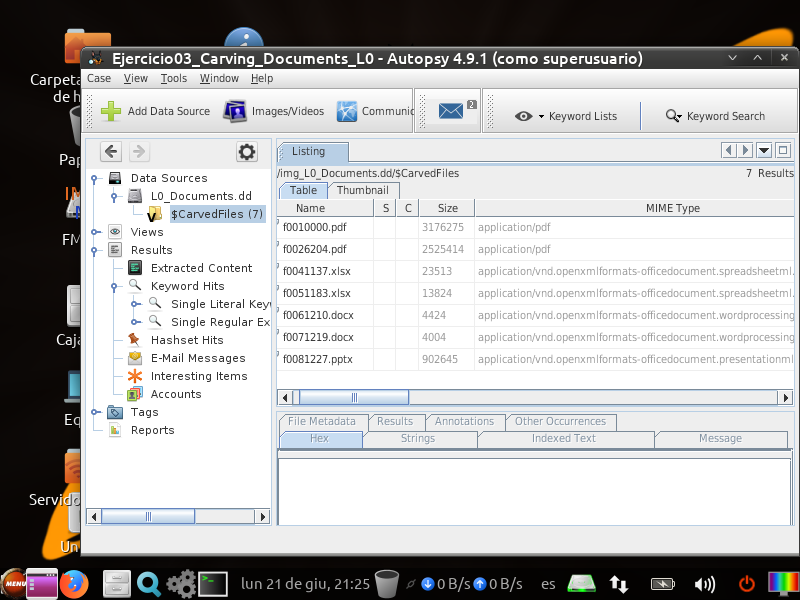
\includegraphics[scale=0.7]{e3-5.png}
\end{figure}

Para obtener las fechas se abren los documentos con las aplicaciones externas correspondientes y se busca en sus propiedades.

\begin{figure}[H]
    \caption{Ejercicio 3: Propiedades del pdf}
    \centering
    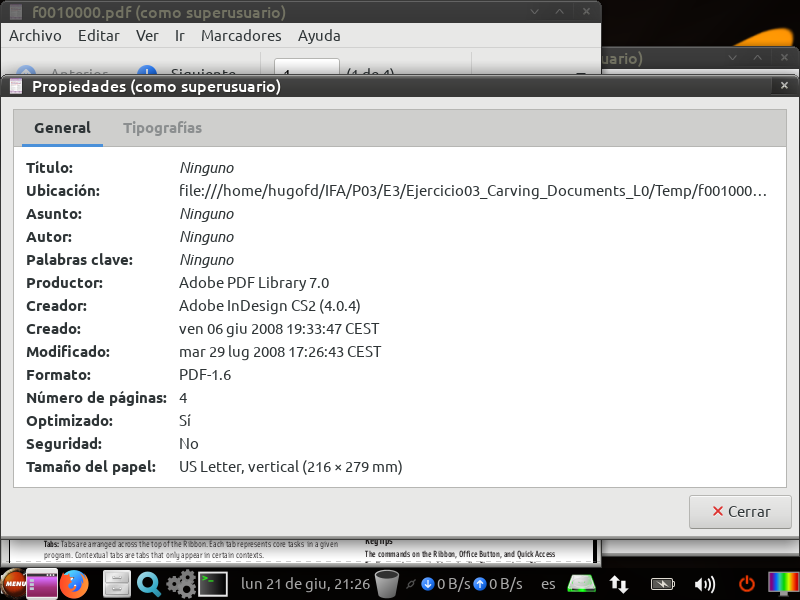
\includegraphics[scale=0.7]{e3-6.png}
\end{figure}

\begin{table}[H]
    \centering
    \begin{tabular}{|p{3cm}|p{2cm}|p{8cm}|p{2cm}|}
        \hline
        Nombre del fichero en Autopsy & Tamaño del fichero (en Bytes) & Tipo MIME documento & Fecha Creación del documento \\
        \hline\hline
        f0010000.pdf & 3176275 & application/pdf & 2008/06/06 \\
        \hline
        f0026204.pdf & 2525414 & application/pdf & 2008/06/04 \\
        \hline
        f0041137.xlsx & 23513 & application/vnd.openxmlformats-officedocument.spreadsheetml.sheet & 2012/06/13 \\
        \hline
        f0051183.xlsx & 13824 & application/vnd.openxmlformats-officedocument.spreadsheetml.sheet & 2012/07/05 \\
        \hline
        f0061210.docx & 4424 & application/vnd.openxmlformats-officedocument.wordprocessingml.document & Sin especificar \\
        \hline
        f0071219.docx & 4004 & application/vnd.openxmlformats-officedocument.wordprocessingml.document & Sin especificar \\
        \hline
        f0081227.pptx & 902645 & application/vnd.openxmlformats-officedocument.presentationml.presentation & 2010/09/28 \\
        \hline
    \end{tabular}
\end{table}

% Ejercicio 4
\section{Ejercicio 4}
Se crea el caso en Autopsy con los datos solicitados.

\begin{figure}[H]
    \caption{Ejercicio 4: Creación del caso}
    \centering
    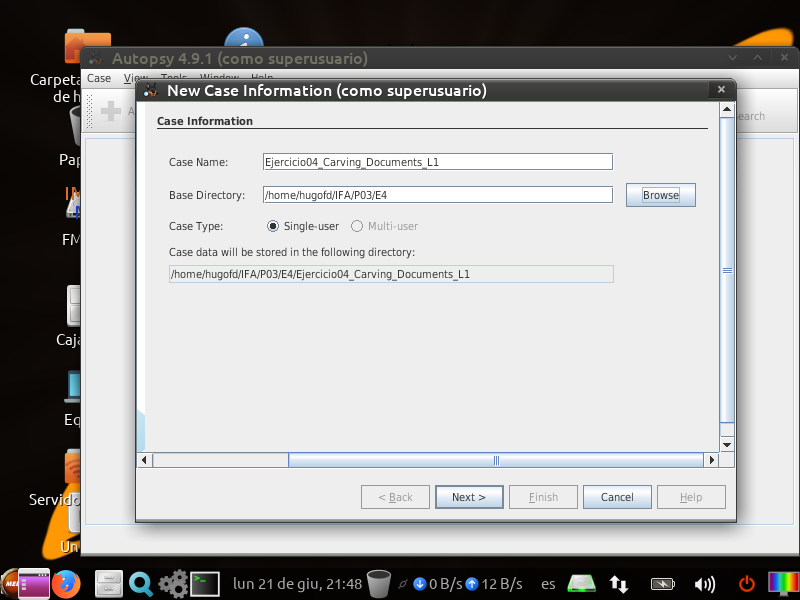
\includegraphics[scale=0.7]{e4-1.png}
\end{figure}

\begin{figure}[H]
    \caption{Ejercicio 4: Detalles del examinador}
    \centering
    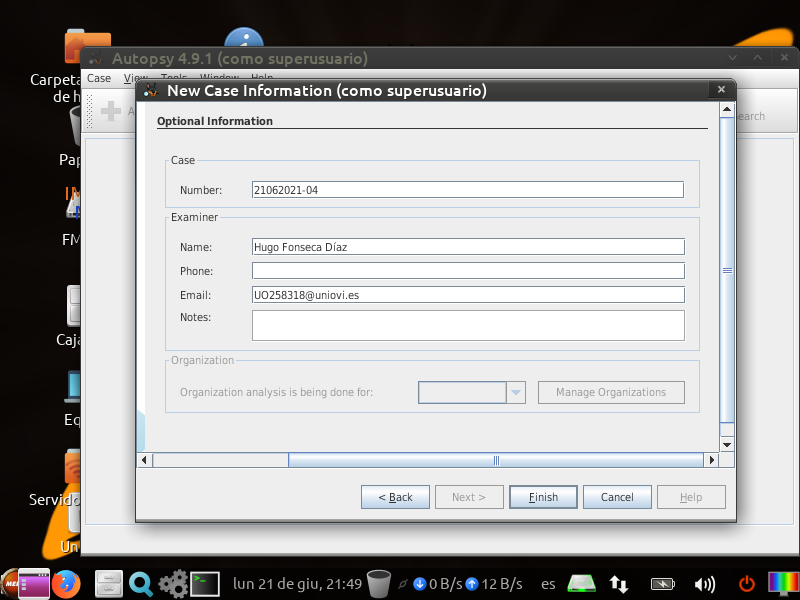
\includegraphics[scale=0.7]{e4-2.png}
\end{figure}

Añadimos la imagen a analizar.

\begin{figure}[H]
    \caption{Ejercicio 4: Selección de la imagen}
    \centering
    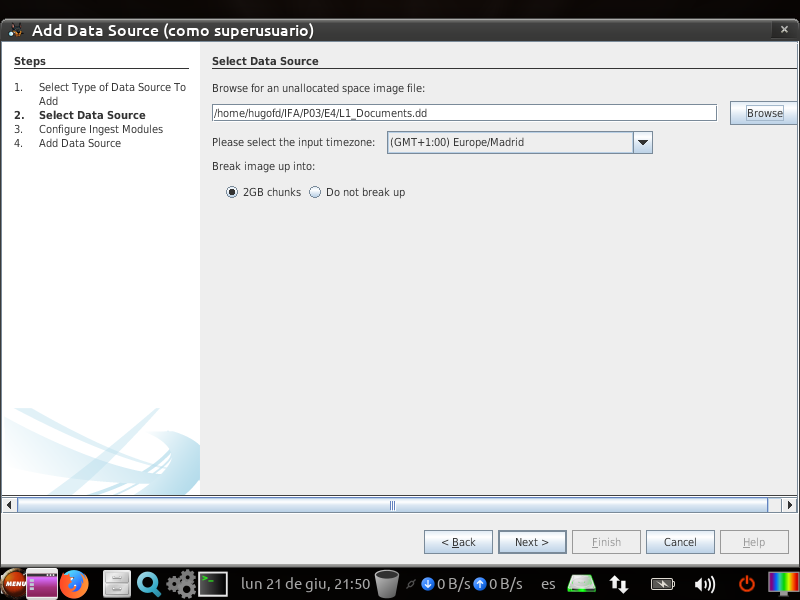
\includegraphics[scale=0.7]{e4-3.png}
\end{figure}

Se seleccionan los módulos de identificación de tipos de fichero, parseador de Exif y \textit{PhotoRec Carver}.

\begin{figure}[H]
    \caption{Ejercicio 4: Selección de módulos}
    \centering
    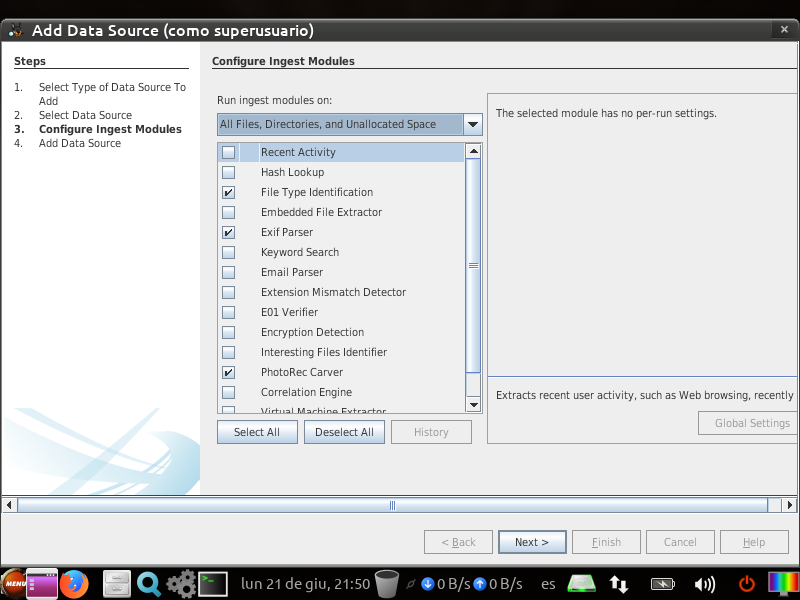
\includegraphics[scale=0.7]{e4-4.png}
\end{figure}

Se ejecuta el análisis y se obtienen los resultados con los que se rellenará la tabla.

\begin{figure}[H]
    \caption{Ejercicio 4: Resultados del análisis}
    \centering
    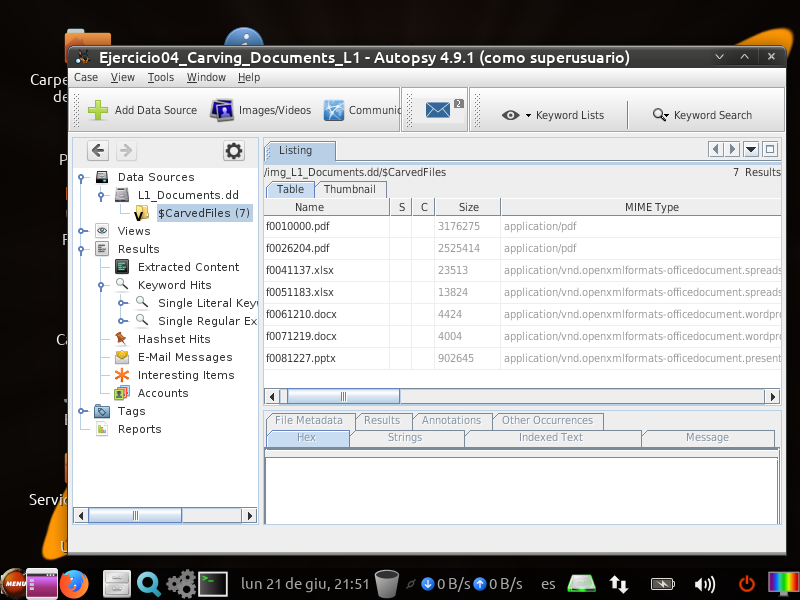
\includegraphics[scale=0.7]{e4-5.png}
\end{figure}

Para obtener las fechas se abren los documentos con las aplicaciones externas correspondientes y se busca en sus propiedades.

\begin{figure}[H]
    \caption{Ejercicio 4: Propiedades del pdf}
    \centering
    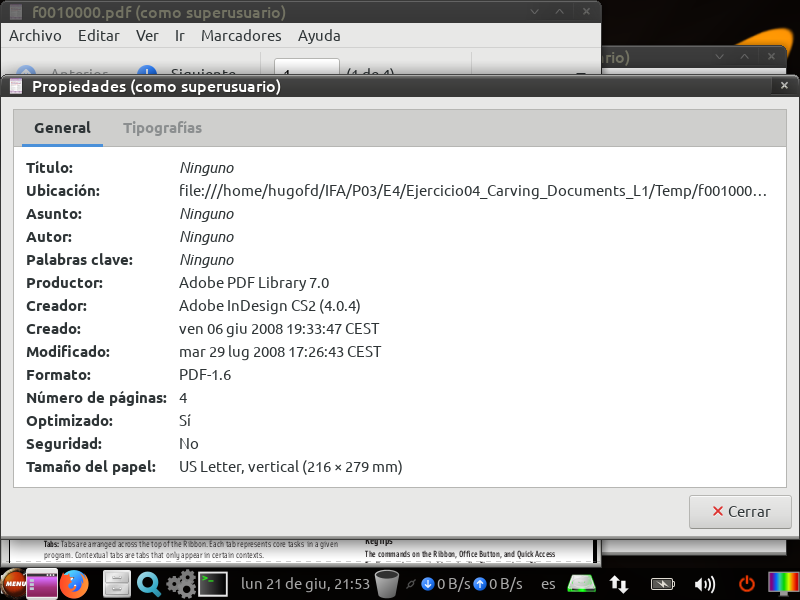
\includegraphics[scale=0.7]{e4-6.png}
\end{figure}

\begin{table}[H]
    \centering
    \begin{tabular}{|p{3cm}|p{2cm}|p{8cm}|p{2cm}|}
        \hline
        Nombre del fichero en Autopsy & Tamaño del fichero (en Bytes) & Tipo MIME documento & Fecha Creación del documento \\
        \hline\hline
        f0010000.pdf & 3176275 & application/pdf & 2008/06/06 \\
        \hline
        f0026204.pdf & 2525414 & application/pdf & 2008/06/04 \\
        \hline
        f0041137.xlsx & 23513 & application/vnd.openxmlformats-officedocument.spreadsheetml.sheet & 2012/06/13 \\
        \hline
        f0051183.xlsx & 13824 & application/vnd.openxmlformats-officedocument.spreadsheetml.sheet & 2012/07/05 \\
        \hline
        f0061210.docx & 4424 & application/vnd.openxmlformats-officedocument.wordprocessingml.document & Sin especificar \\
        \hline
        f0071219.docx & 4004 & application/vnd.openxmlformats-officedocument.wordprocessingml.document & Sin especificar \\
        \hline
        f0081227.pptx & 902645 & application/vnd.openxmlformats-officedocument.presentationml.presentation & 2010/09/28 \\
        \hline
    \end{tabular}
\end{table}

% Ejercicio 5
\section{Ejercicio 5}
Se crea el caso en Autopsy con los datos solicitados.

\begin{figure}[H]
    \caption{Ejercicio 5: Creación del caso}
    \centering
    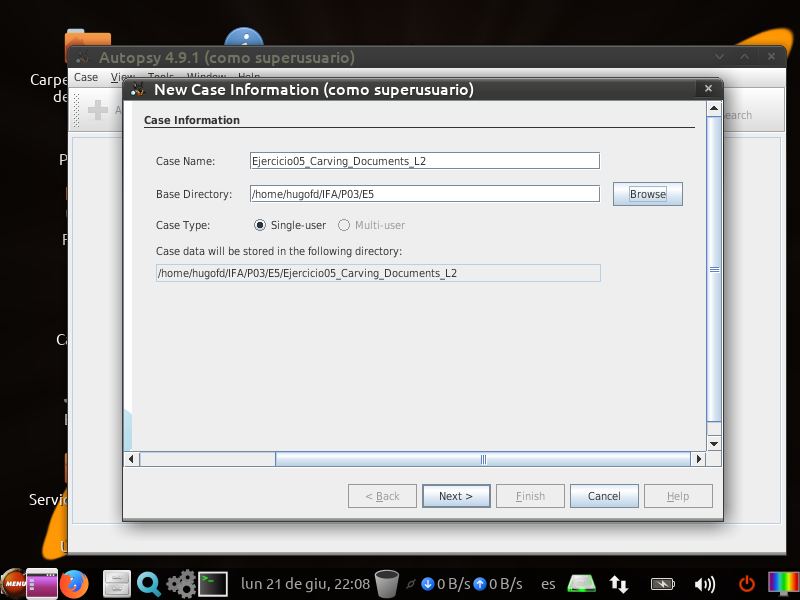
\includegraphics[scale=0.7]{e5-1.png}
\end{figure}

\begin{figure}[H]
    \caption{Ejercicio 5: Detalles del examinador}
    \centering
    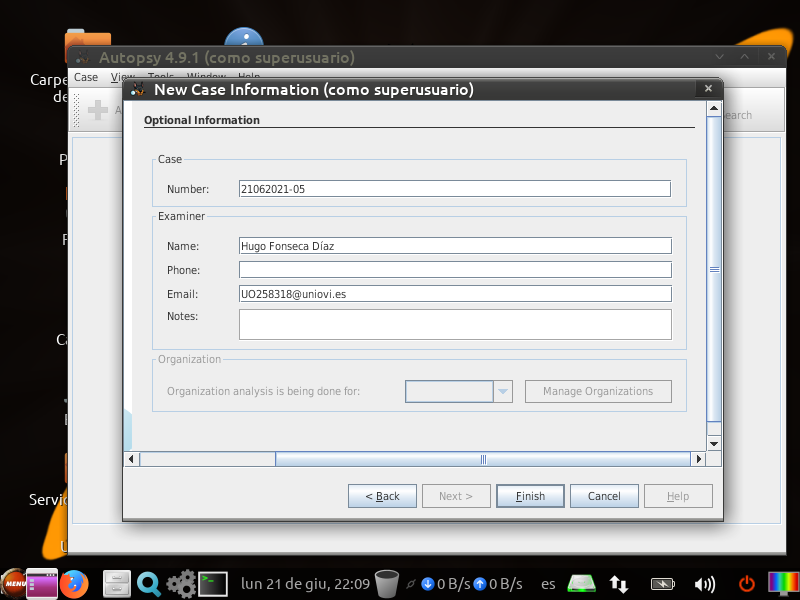
\includegraphics[scale=0.7]{e5-2.png}
\end{figure}

Añadimos la imagen a analizar.

\begin{figure}[H]
    \caption{Ejercicio 5: Selección de la imagen}
    \centering
    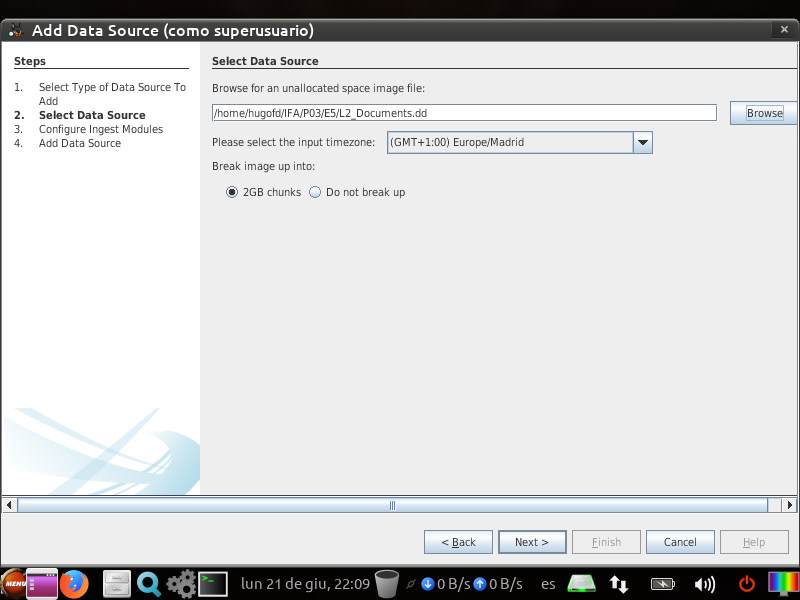
\includegraphics[scale=0.7]{e5-3.png}
\end{figure}

Se seleccionan los módulos de identificación de tipos de fichero, parseador de Exif y \textit{PhotoRec Carver}.

\begin{figure}[H]
    \caption{Ejercicio 5: Selección de módulos}
    \centering
    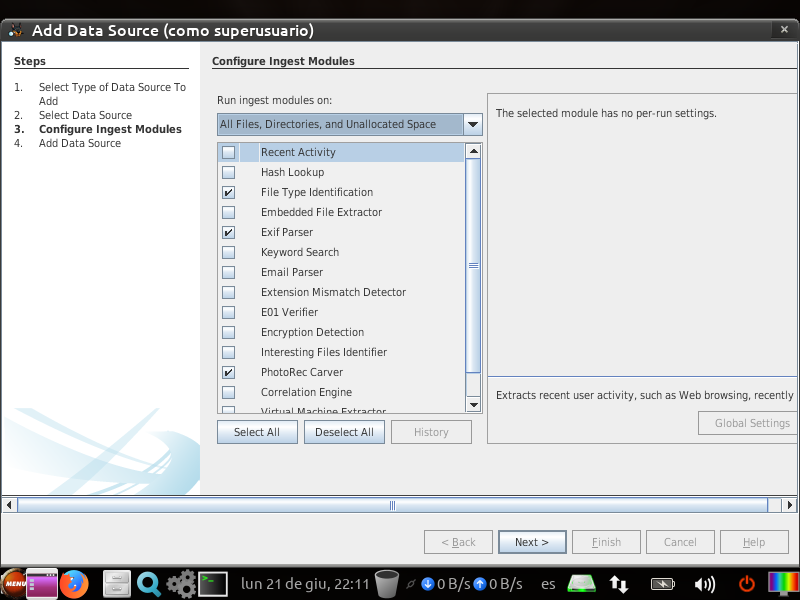
\includegraphics[scale=0.7]{e5-4.png}
\end{figure}

Se ejecuta el análisis y se obtienen los resultados con los que se responderá a las preguntas.

\begin{figure}[H]
    \caption{Ejercicio 5: Resultados del análisis}
    \centering
    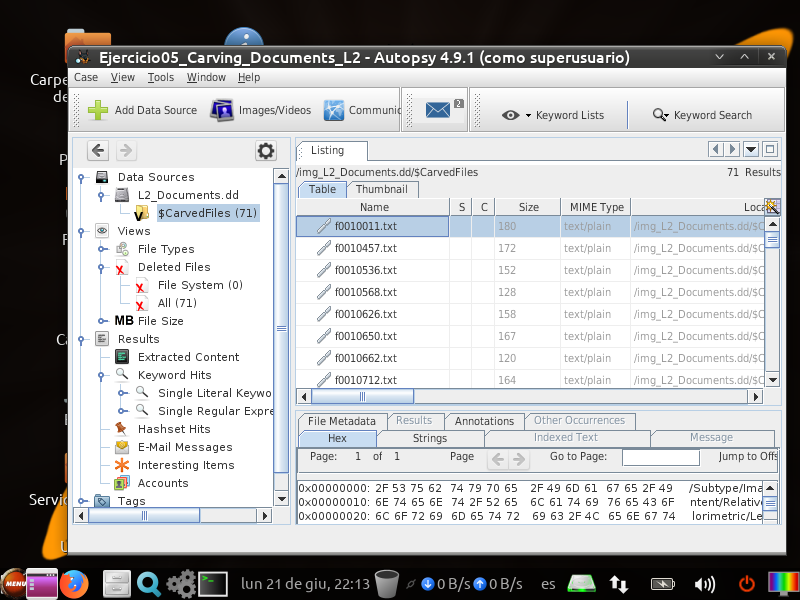
\includegraphics[scale=0.7]{e5-5.png}
\end{figure}

a) Hay 71 falsos positivos.

b) Todos son de tipo texto plano.

Esto puede deberse a que Autopsy no haya sido capaz de recuperar los archivos con sus verdaderos tipos MIME y los fragmentos de esos archivos sean tratados como texto plano.

% Ejercicio 6
\section{Ejercicio 6}
Se crea el caso en Autopsy con los datos solicitados.

\begin{figure}[H]
    \caption{Ejercicio 6: Creación del caso}
    \centering
    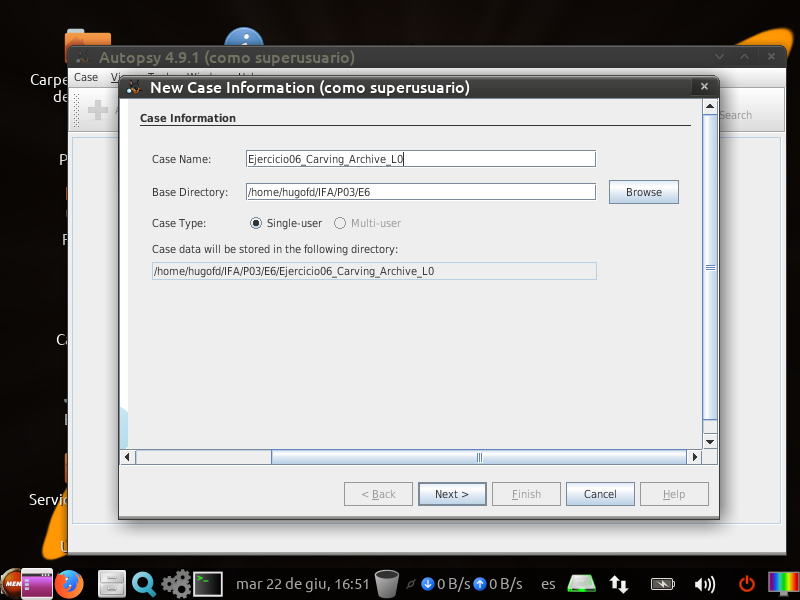
\includegraphics[scale=0.7]{e6-1.png}
\end{figure}

\begin{figure}[H]
    \caption{Ejercicio 6: Detalles del examinador}
    \centering
    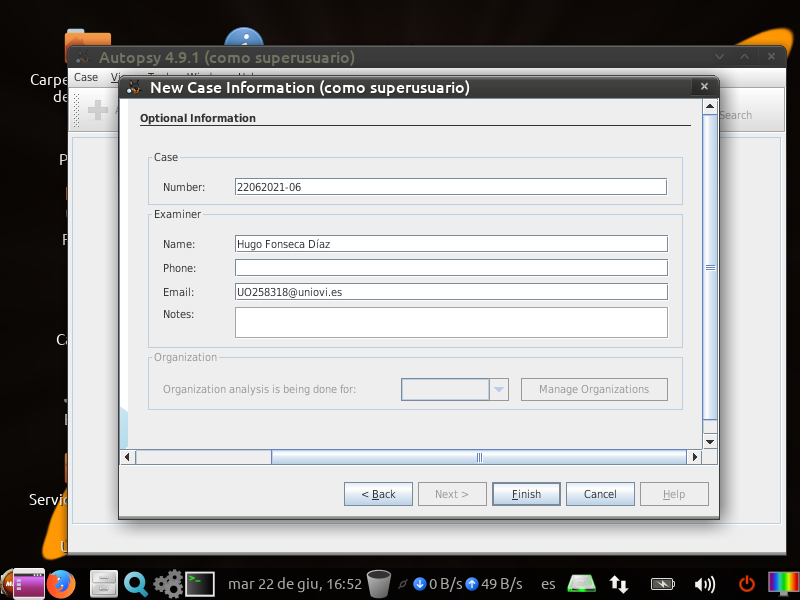
\includegraphics[scale=0.7]{e6-2.png}
\end{figure}

Añadimos la imagen a analizar.

\begin{figure}[H]
    \caption{Ejercicio 6: Selección de la imagen}
    \centering
    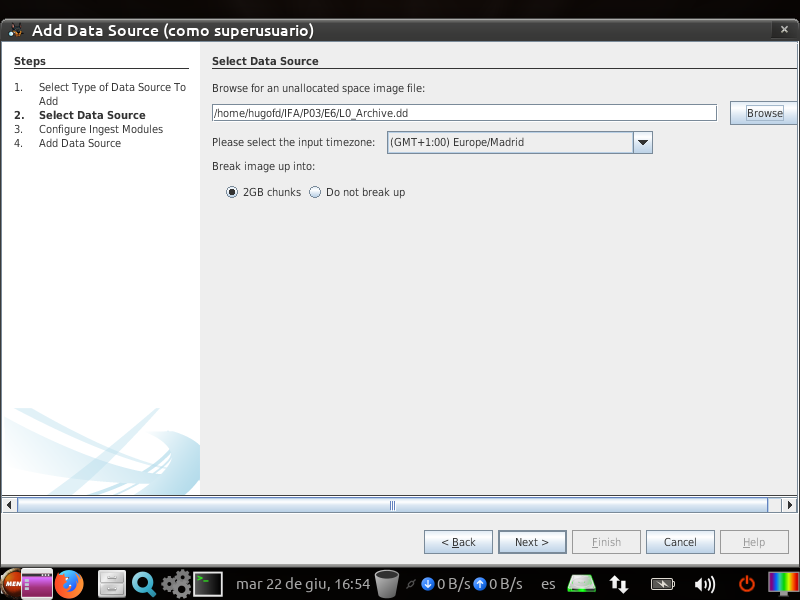
\includegraphics[scale=0.7]{e6-3.png}
\end{figure}

Se seleccionan los módulos de identificación de tipos de fichero, parseador de Exif, \textit{PhotoRec Carver} y el módulo de extracción de ficheros.

\begin{figure}[H]
    \caption{Ejercicio 6: Selección de módulos}
    \centering
    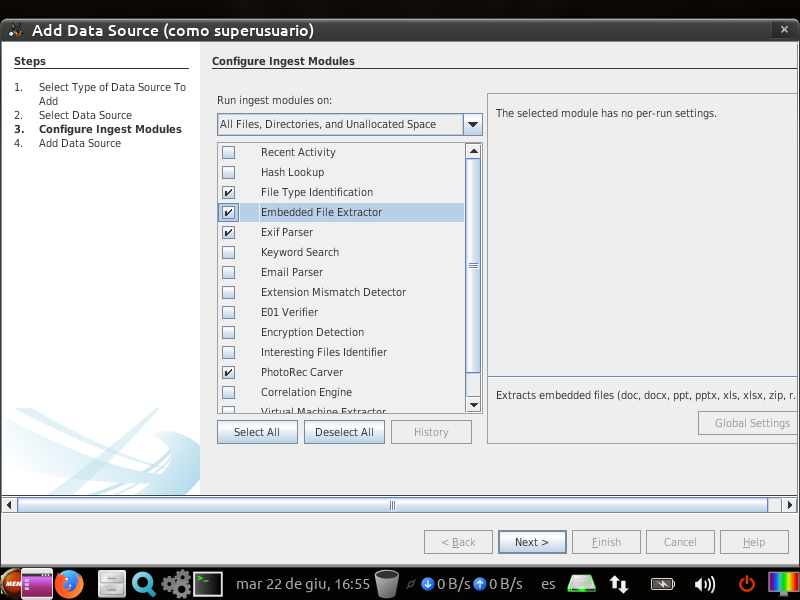
\includegraphics[scale=0.7]{e6-4.png}
\end{figure}

Se ejecuta el análisis y se obtienen los resultados con los que se rellenará la tabla.

\begin{figure}[H]
    \caption{Ejercicio 6: Resultados del análisis}
    \centering
    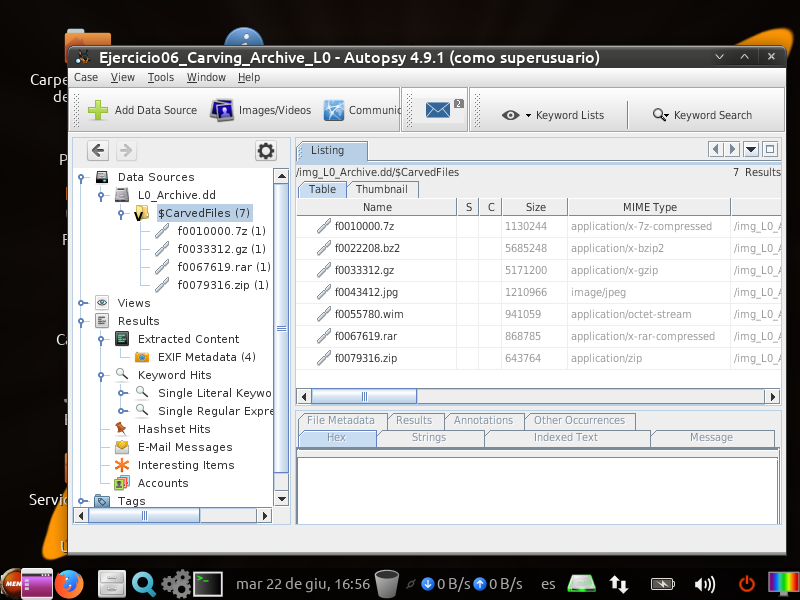
\includegraphics[scale=0.7]{e6-5.png}
\end{figure}

TBD table.

Se extraen las imágenes de los ficheros comprimidos.

\begin{figure}[H]
    \caption{Ejercicio 6: Imágenes extraídas}
    \centering
    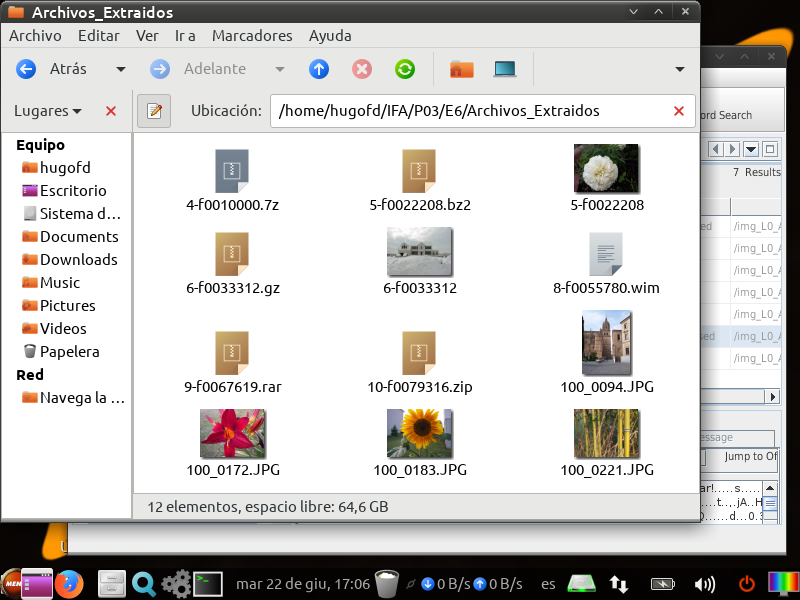
\includegraphics[scale=0.7]{e6-6.png}
\end{figure}

Se ejecuta la herramienta \textit{exiftool} para obtener los datos que se usan a la hora de rellenar la siguiente tabla.

\begin{figure}[H]
    \caption{Ejercicio 6: Resultado del comando \textit{exiftool} con una de las imágenes extraídas}
    \centering
    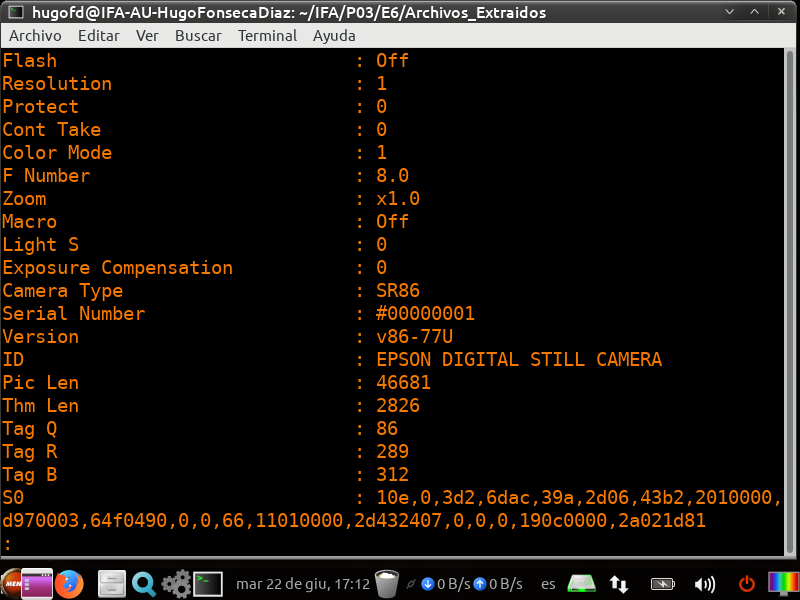
\includegraphics[scale=0.7]{e6-7.png}
\end{figure}

TBD table.

% Ejercicio 7
\section{Ejercicio 7}
Se crea el caso en Autopsy con los datos solicitados.

\begin{figure}[H]
    \caption{Ejercicio 7: Creación del caso}
    \centering
    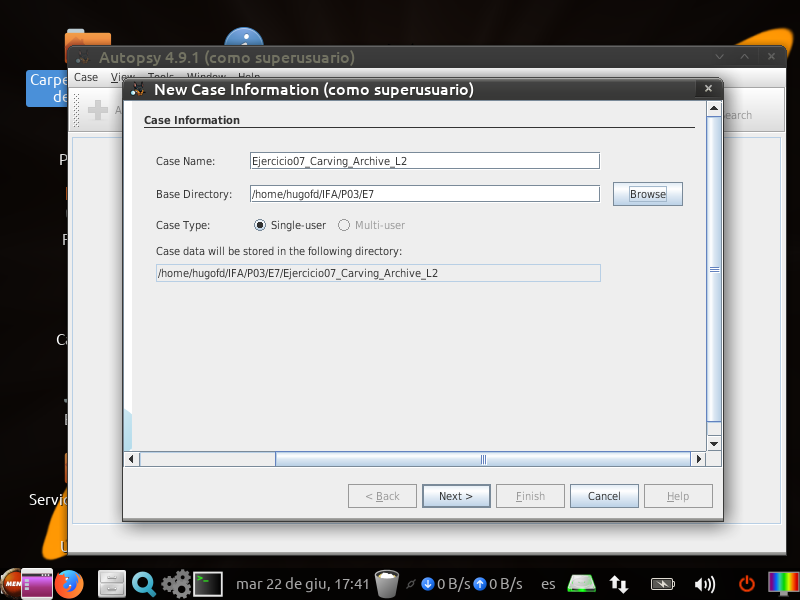
\includegraphics[scale=0.7]{e7-1.png}
\end{figure}

\begin{figure}[H]
    \caption{Ejercicio 7: Detalles del examinador}
    \centering
    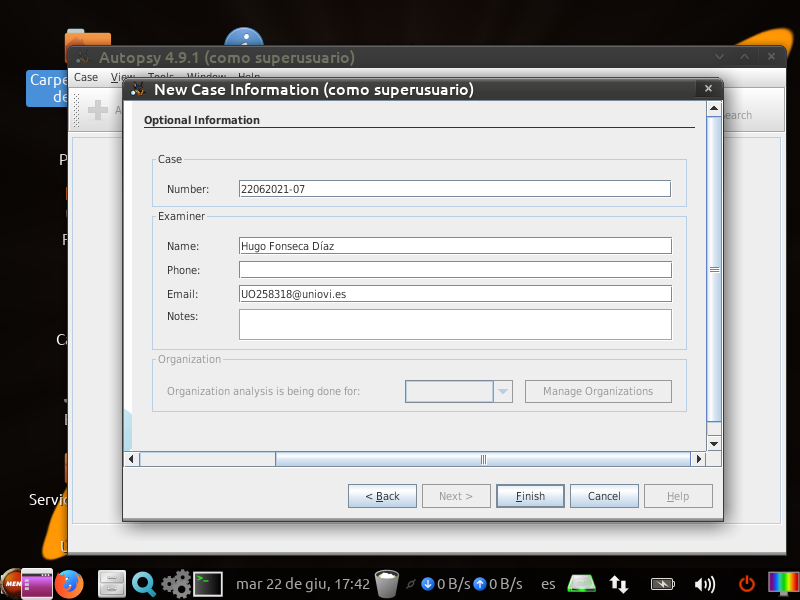
\includegraphics[scale=0.7]{e7-2.png}
\end{figure}

Añadimos la imagen a analizar.

\begin{figure}[H]
    \caption{Ejercicio 7: Selección de la imagen}
    \centering
    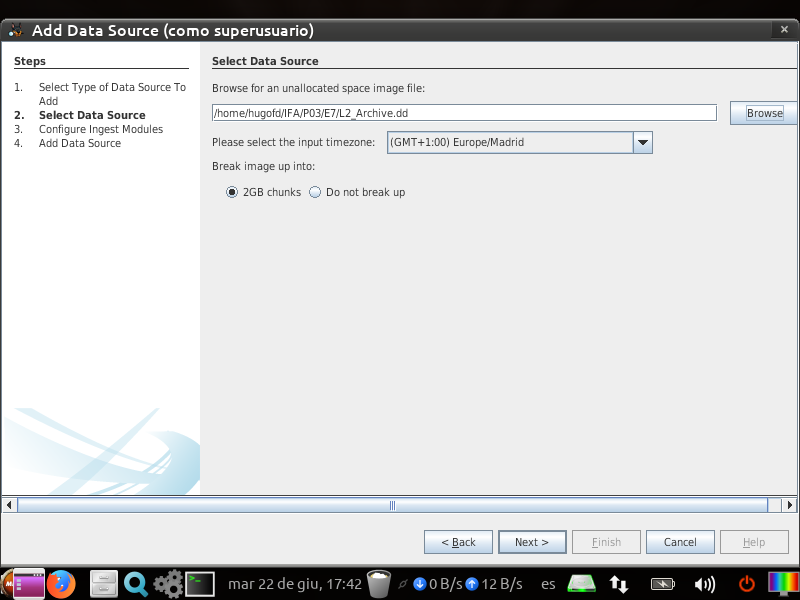
\includegraphics[scale=0.7]{e7-3.png}
\end{figure}

Se seleccionan los módulos de identificación de tipos de fichero, parseador de Exif, \textit{PhotoRec Carver} y el módulo de extracción de ficheros.

\begin{figure}[H]
    \caption{Ejercicio 7: Selección de módulos}
    \centering
    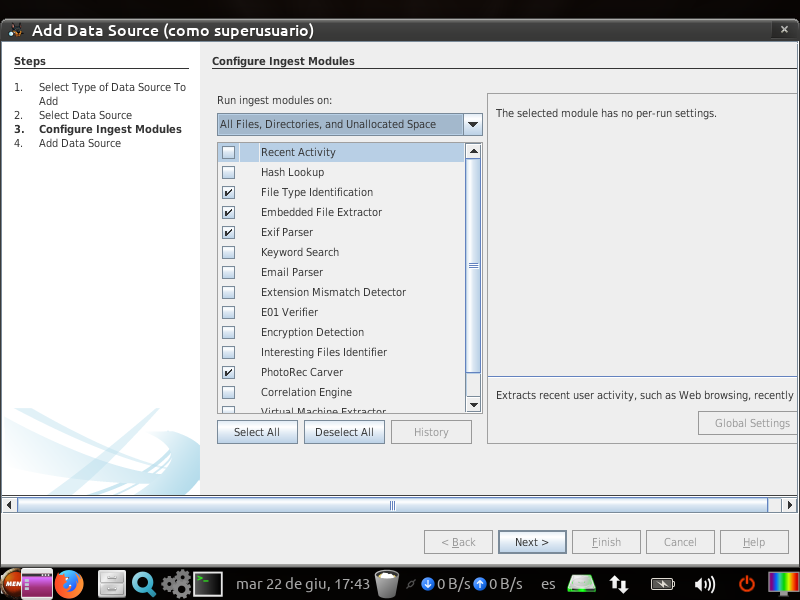
\includegraphics[scale=0.7]{e7-4.png}
\end{figure}

Se ejecuta el análisis y se observa que Autopsy ha detectado una posible bomba zip entre uno de los ficheros comprimidos.

\begin{figure}[H]
    \caption{Ejercicio 7: Resultados del análisis}
    \centering
    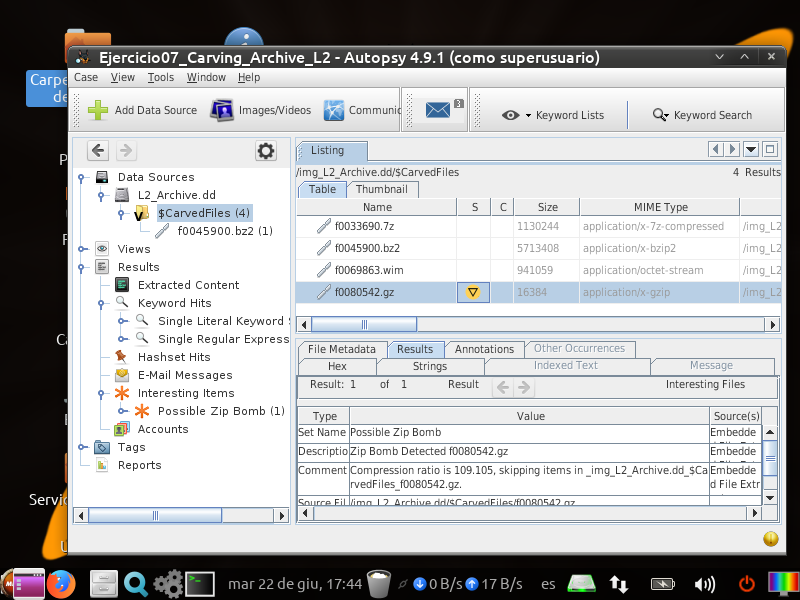
\includegraphics[scale=0.7]{e7-5.png}
\end{figure}

Se instalan los paquetes \textit{clamav} y \textit{clamtk} y se analiza la carpeta donde se extrayeron los ficheros comprimidos.

\begin{figure}[H]
    \caption{Ejercicio 7: Instalación de \textit{clamav} y \textit{clamtk}}
    \centering
    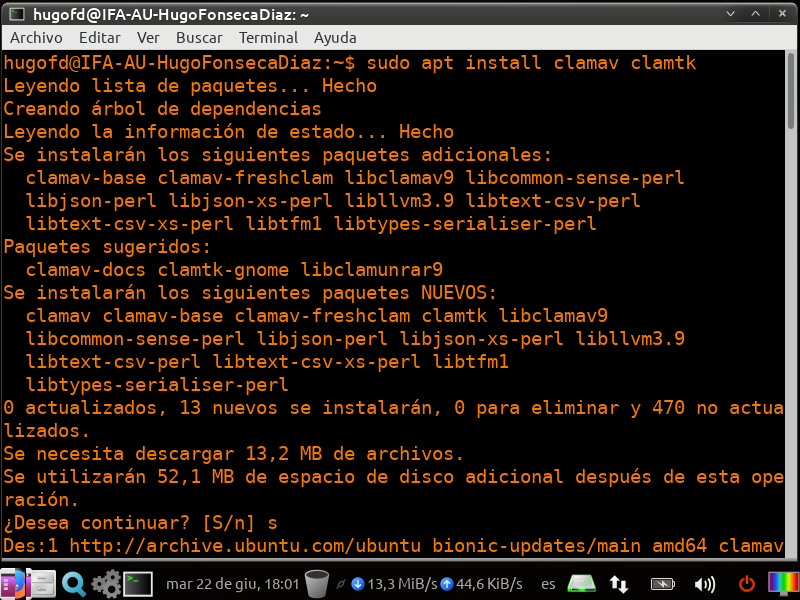
\includegraphics[scale=0.7]{e7-6.png}
\end{figure}

\begin{figure}[H]
    \caption{Ejercicio 7: Resultados del análisis del antivirus}
    \centering
    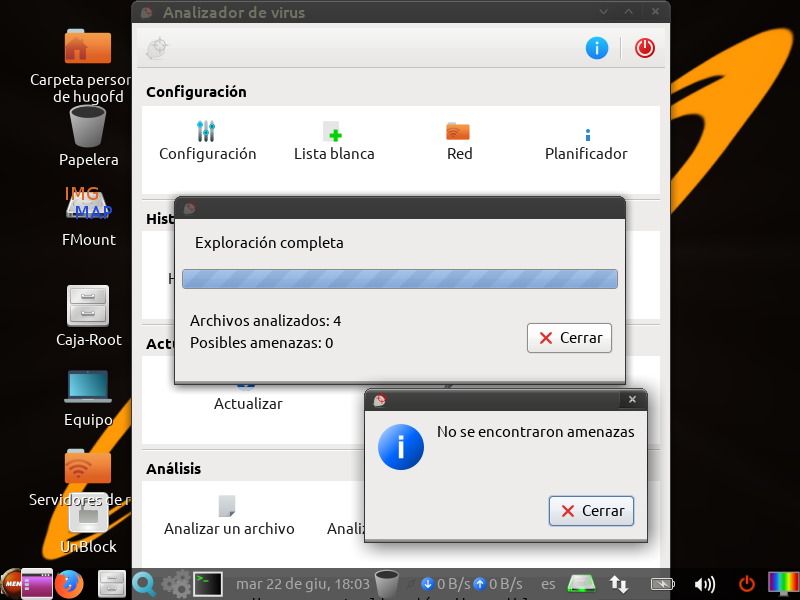
\includegraphics[scale=0.7]{e7-7.png}
\end{figure}

a) El antivirus no detecta nada, pero Autopsy si que notificó que uno de los ficheros podía ser una bomba zip. Este es un ataque que comprime con una alta proporción una gran cantidad de datos en un archivo comprimido de pocos datos. Sirve para inutilizar los programas que descomprimem dicho fichero, normalmente se busca inutilizar un antivirus, para luego ejecutar otro tipo de malware.

b) Bomba zip.

% Ejercicio 8
\section{Ejercicio 8}
Se crea el caso en Autopsy con los datos solicitados.

\begin{figure}[H]
    \caption{Ejercicio 8: Creación del caso}
    \centering
    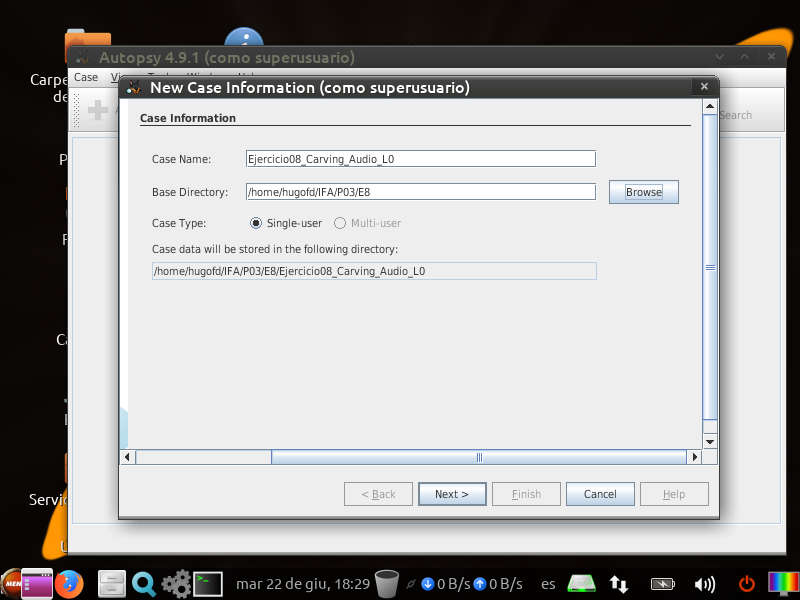
\includegraphics[scale=0.7]{e8-1.png}
\end{figure}

\begin{figure}[H]
    \caption{Ejercicio 8: Detalles del examinador}
    \centering
    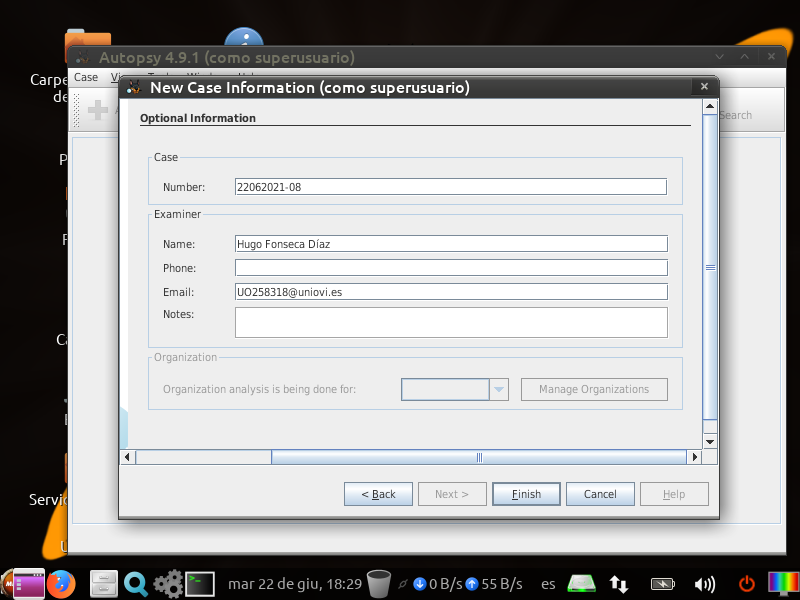
\includegraphics[scale=0.7]{e8-2.png}
\end{figure}

Añadimos la imagen a analizar.

\begin{figure}[H]
    \caption{Ejercicio 8: Selección de la imagen}
    \centering
    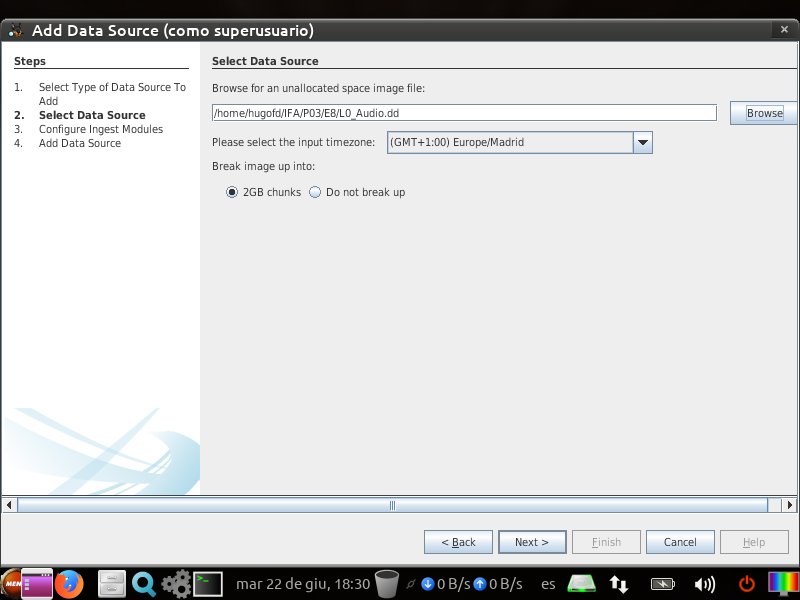
\includegraphics[scale=0.7]{e8-3.png}
\end{figure}

Se seleccionan los módulos de identificación de tipos de fichero, parseador de Exif y \textit{PhotoRec Carver}.

\begin{figure}[H]
    \caption{Ejercicio 8: Selección de módulos}
    \centering
    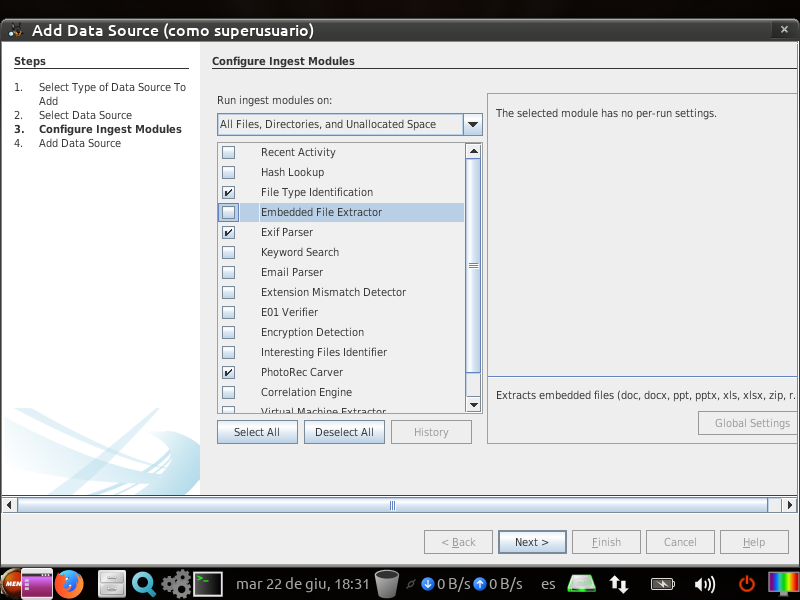
\includegraphics[scale=0.7]{e8-4.png}
\end{figure}

Para rellenar la tabla se usarán los datos obtenidos al ejecutar el análisis de Autopsy y mediante el uso de la herramienta \textit{MediaInfo}.

\begin{figure}[H]
    \caption{Ejercicio 8: Resultados del análisis}
    \centering
    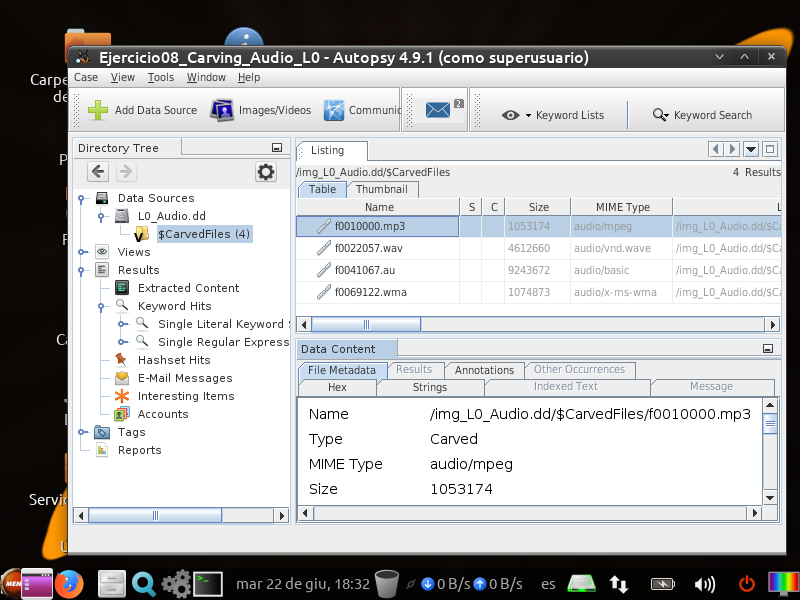
\includegraphics[scale=0.7]{e8-5.png}
\end{figure}

\begin{figure}[H]
    \caption{Ejercicio 8: Herramienta \textit{MediaInfo}}
    \centering
    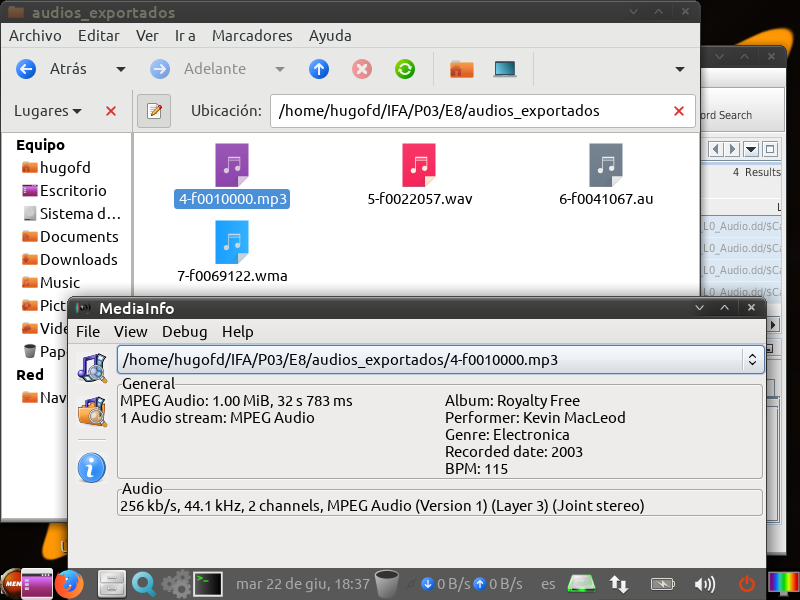
\includegraphics[scale=0.7]{e8-6.png}
\end{figure}

TBD table.

% Ejercicio 9
\section{Ejercicio 9}
Se crea el caso en Autopsy con los datos solicitados.

\begin{figure}[H]
    \caption{Ejercicio 9: Creación del caso}
    \centering
    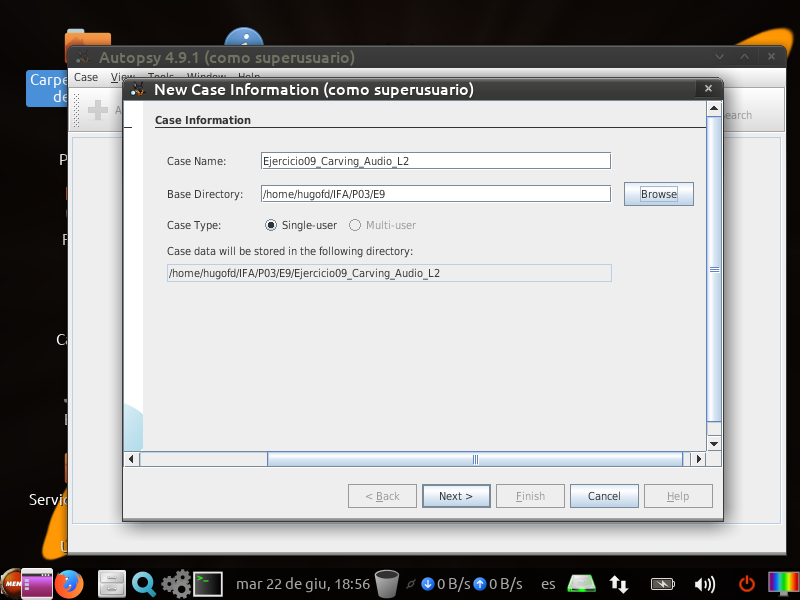
\includegraphics[scale=0.7]{e9-1.png}
\end{figure}

\begin{figure}[H]
    \caption{Ejercicio 9: Detalles del examinador}
    \centering
    \includegraphics[scale=0.7]{e9-2.png}
\end{figure}

Añadimos la imagen a analizar.

\begin{figure}[H]
    \caption{Ejercicio 9: Selección de la imagen}
    \centering
    \includegraphics[scale=0.7]{e9-3.png}
\end{figure}

Se seleccionan los módulos de identificación de tipos de fichero, parseador de Exif y \textit{PhotoRec Carver}.

\begin{figure}[H]
    \caption{Ejercicio 9: Selección de módulos}
    \centering
    \includegraphics[scale=0.7]{e9-4.png}
\end{figure}

Para rellenar la tabla se usarán los datos obtenidos al ejecutar el análisis de Autopsy y mediante el uso de la herramienta \textit{MediaInfo}.

\begin{figure}[H]
    \caption{Ejercicio 9: Resultados del análisis}
    \centering
    \includegraphics[scale=0.7]{e9-5.png}
\end{figure}

\begin{figure}[H]
    \caption{Ejercicio 9: Herramienta \textit{MediaInfo}}
    \centering
    \includegraphics[scale=0.7]{e9-6.png}
\end{figure}

TBD table.

% Ejercicio 10
\section{Ejercicio 10}
Se crea el caso en Autopsy con los datos solicitados.

\begin{figure}[H]
    \caption{Ejercicio 10: Creación del caso}
    \centering
    \includegraphics[scale=0.7]{e10-1.png}
\end{figure}

\begin{figure}[H]
    \caption{Ejercicio 10: Detalles del examinador}
    \centering
    \includegraphics[scale=0.7]{e10-2.png}
\end{figure}

Añadimos la imagen a analizar.

\begin{figure}[H]
    \caption{Ejercicio 10: Selección de la imagen}
    \centering
    \includegraphics[scale=0.7]{e10-3.png}
\end{figure}

Se seleccionan los módulos de identificación de tipos de fichero, parseador de Exif y \textit{PhotoRec Carver}.

\begin{figure}[H]
    \caption{Ejercicio 10: Selección de módulos}
    \centering
    \includegraphics[scale=0.7]{e10-4.png}
\end{figure}

Para rellenar la tabla se usarán los datos obtenidos al ejecutar el análisis de Autopsy y mediante el uso de las herramientas \textit{MediaInfo} y \textit{FileInfo}.

\begin{figure}[H]
    \caption{Ejercicio 10: Resultados del análisis}
    \centering
    \includegraphics[scale=0.7]{e10-5.png}
\end{figure}

\begin{figure}[H]
    \caption{Ejercicio 10: Herramienta \textit{FileInfo}}
    \centering
    \includegraphics[scale=0.7]{e10-6.png}
\end{figure}

TBD table.

% Ejercicio 11
\section{Ejercicio 11}
Para realizar la primera parte del ejercicio se utilizará el comando \verb|xxd| junto al comando \verb|grep|. Empezamos buscando la cadena \textit{JFIF} en la imagen del ejercicio. Con esta búsqueda se sacará el offset en hexadecimal, y se convertirá a decimal en \textit{bash}.

\begin{figure}[H]
    \caption{Ejercicio 11: \textit{xxd} con una pipe a \textit{grep}}
    \centering
    \includegraphics[scale=0.7]{e11-1.png}
\end{figure}

Una vez obtenido el offset, se buscará el final de la imagen. Para ello se buscará con \verb|grep| la cadena \textit{ffd9} pasándole al comando \verb|xxd| el offset obtenido previamente.

\begin{figure}[H]
    \caption{Ejercicio 11: Buscando el final de la imagen}
    \centering
    \includegraphics[scale=0.7]{e11-2.png}
\end{figure}

Una vez se ha encontrado el offset del final de la imagen, se le suma el desplazamiento, en este caso 10 bytes, y se calcula el tamaño restando el offset final del inicial.

\begin{figure}[H]
    \caption{Ejercicio 11: Calculando tamaño de imagen}
    \centering
    \includegraphics[scale=0.7]{e11-3.png}
\end{figure}

Ahora se utiliza el comando \verb|dd| con la información obtenida previamente y se comprueba que la imagen extraída es la del cartel que pone 'Welcome to Moscow'.

\begin{figure}[H]
    \caption{Ejercicio 11: Carving de la imagen}
    \centering
    \includegraphics[scale=0.7]{e11-4.png}
\end{figure}

% Ejercicio 12
\section{Ejercicio 12}
Se crea el caso en Autopsy con los datos solicitados.

\begin{figure}[H]
    \caption{Ejercicio 12: Creación del caso}
    \centering
    \includegraphics[scale=0.7]{e12-1.png}
\end{figure}

\begin{figure}[H]
    \caption{Ejercicio 12: Detalles del examinador}
    \centering
    \includegraphics[scale=0.7]{e12-2.png}
\end{figure}

Añadimos la imagen a analizar.

\begin{figure}[H]
    \caption{Ejercicio 12: Selección de la imagen}
    \centering
    \includegraphics[scale=0.7]{e12-3.png}
\end{figure}

Se seleccionan los módulos de identificación de tipos de fichero y \textit{PhotoRec Carver}.

\begin{figure}[H]
    \caption{Ejercicio 12: Selección de módulos}
    \centering
    \includegraphics[scale=0.7]{e12-4.png}
\end{figure}

Se obtienen los resultados del análisis con los que se responderán a las diferentes cuestiones del ejercicio.

\begin{figure}[H]
    \caption{Ejercicio 12: Resultados del análisis}
    \centering
    \includegraphics[scale=0.7]{e12-5.png}
\end{figure}

a) TBD table

b) Para responder a esta cuestión se observan los resultados de la pestaña 'Views'.

\begin{figure}[H]
    \caption{Ejercicio 12: Ficheros de texto plano}
    \centering
    \includegraphics[scale=0.7]{e12-6.png}
\end{figure}

Se puede ver que hay 9 ficheros de texto plano, 3 de ellos borrados.

c) Para rellenar esta tabla se miran los metadatos que muestra Autopsy de cada archivo borrado.

\begin{figure}[H]
    \caption{Ejercicio 12: Metadatos de los ficheros borrados}
    \centering
    \includegraphics[scale=0.7]{e12-7.png}
\end{figure}

TBD table

d) Se muestran a continuación las líneas de tiempo de los tres ficheros borrados, en el filtro de la parte izquierda de la captura se observa el fichero actual.

\begin{figure}[H]
    \caption{Ejercicio 12: Línea temporal de \textit{Bellatrix.txt}}
    \centering
    \includegraphics[scale=0.7]{e12-8.png}
\end{figure}

\begin{figure}[H]
    \caption{Ejercicio 12: Línea temporal de \textit{\_BEID.txt}}
    \centering
    \includegraphics[scale=0.7]{e12-9.png}
\end{figure}

\begin{figure}[H]
    \caption{Ejercicio 12: Línea temporal de \textit{Betelgeuse.txt}}
    \centering
    \includegraphics[scale=0.7]{e12-10.png}
\end{figure}



% Bibliografía
\begin{thebibliography}{8}
\end{thebibliography}

\end{document}


